%% BioMed_Central_Tex_Template_v1.06
%%                                      %
%  bmc_article.tex            ver: 1.06 %
%                                       %
%%IMPORTANT: do not delete the first line of this template
%%It must be present to enable the BMC Submission system to
%%recognise this template!!

%%%%%%%%%%%%%%%%%%%%%%%%%%%%%%%%%%%%%%%%%
%%                                     %%
%%  LaTeX template for BioMed Central  %%
%%     journal article submissions     %%
%%                                     %%
%%          <8 June 2020>              %%
%%                                     %%
%%                                     %%
%%%%%%%%%%%%%%%%%%%%%%%%%%%%%%%%%%%%%%%%%

%%%%%%%%%%%%%%%%%%%%%%%%%%%%%%%%%%%%%%%%%%%%%%%%%%%%%%%%%%%%%%%%%%%%%
%%                                                                 %%
%% For instructions on how to fill out this Tex template           %%
%% document please refer to Readme.html and the instructions for   %%
%% authors page on the biomed central website                      %%
%% https://www.biomedcentral.com/getpublished                      %%
%%                                                                 %%
%% Please do not use \input{...} to include other tex files.       %%
%% Submit your LaTeX manuscript as one .tex document.              %%
%%                                                                 %%
%% All additional figures and files should be attached             %%
%% separately and not embedded in the \TeX\ document itself.       %%
%%                                                                 %%
%% BioMed Central currently use the MikTex distribution of         %%
%% TeX for Windows) of TeX and LaTeX.  This is available from      %%
%% https://miktex.org/                                             %%
%%                                                                 %%
%%%%%%%%%%%%%%%%%%%%%%%%%%%%%%%%%%%%%%%%%%%%%%%%%%%%%%%%%%%%%%%%%%%%%

%%% additional documentclass options:
%  [doublespacing]
%  [linenumbers]   - put the line numbers on margins

%%% loading packages, author definitions

%\documentclass[twocolumn]{bmcart}% uncomment this for twocolumn layout and comment line below
\documentclass{bmcart}
\usepackage{hyperref}

%%% Load packages
\usepackage{tabularx}
\usepackage{multirow}
\usepackage{lscape}
\usepackage{rotating}
\usepackage{amsthm,amsmath}
%\RequirePackage[authoryear]{natbib}% uncomment this for author-year bibliography
%\RequirePackage{hyperref}
\usepackage{graphicx}
\usepackage[utf8]{inputenc} %unicode support
%\usepackage[applemac]{inputenc} %applemac support if unicode package fails
%\usepackage[latin1]{inputenc} %UNIX support if unicode package fails
\usepackage{algorithm}
\usepackage{algorithmic}
\renewcommand{\algorithmiccomment}[1]{$\triangleright$ #1}
%%%%%%%%%%%%%%%%%%%%%%%%%%%%%%%%%%%%%%%%%%%%%%%%%
%%                                             %%
%%  If you wish to display your graphics for   %%
%%  your own use using includegraphic or       %%
%%  includegraphics, then comment out the      %%
%%  following two lines of code.               %%
%%  NB: These line *must* be included when     %%
%%  submitting to BMC.                         %%
%%  All figure files must be submitted as      %%
%%  separate graphics through the BMC          %%
%%  submission process, not included in the    %%
%%  submitted article.                         %%
%%                                             %%
%%%%%%%%%%%%%%%%%%%%%%%%%%%%%%%%%%%%%%%%%%%%%%%%%

%\def\includegraphic{}
%\def\includegraphics{}

%%% Put your definitions there:
\startlocaldefs
\endlocaldefs

%%% Begin ...
\begin{document}

%%% Start of article front matter
\begin{frontmatter}

\begin{fmbox}
\dochead{Research}

%%%%%%%%%%%%%%%%%%%%%%%%%%%%%%%%%%%%%%%%%%%%%%
%%                                          %%
%% Enter the title of your article here     %%
%%                                          %%
%%%%%%%%%%%%%%%%%%%%%%%%%%%%%%%%%%%%%%%%%%%%%%

\title{Predicting Comperhensive Drug - Drug Interaction via Similarity Network Fusion and Convolutional Neural Networks}

%%%%%%%%%%%%%%%%%%%%%%%%%%%%%%%%%%%%%%%%%%%%%%
%%                                          %%
%% Enter the authors here                   %%
%%                                          %%
%% Specify information, if available,       %%
%% in the form:                             %%
%%   <key>={<id1>,<id2>}                    %%
%%   <key>=                                 %%
%% Comment or delete the keys which are     %%
%% not used. Repeat \author command as much %%
%% as required.                             %%
%%                                          %%
%%%%%%%%%%%%%%%%%%%%%%%%%%%%%%%%%%%%%%%%%%%%%%
\author[
  addressref={aff1,aff2},
  email={khodamoradi1992@gmail.com}
]{\inits{M.A.K.}\fnm{Mohammad.Amin} \snm{Khodamoradi}}
\author[
  addressref={aff1,aff2},
  email={Bahar.levian@gmail.com}
]{\inits{B.L.}\fnm{Bahareh} \snm{Levian}}
\author[
  addressref={aff1,aff2},                   % id's of addresses, e.g. {aff1,aff2}
  corref={aff1},                       % id of corresponding address, if any
% noteref={n1},                        % id's of article notes, if any
  email={eslahchi.ch@gmail.com}   % email address
]{\inits{C.E.}\fnm{Changiz} \snm{Eslahchi}}


%%%%%%%%%%%%%%%%%%%%%%%%%%%%%%%%%%%%%%%%%%%%%%
%%                                          %%
%% Enter the authors' addresses here        %%
%%                                          %%
%% Repeat \address commands as much as      %%
%% required.                                %%
%%                                          %%
%%%%%%%%%%%%%%%%%%%%%%%%%%%%%%%%%%%%%%%%%%%%%%

\address[id=aff1]{%                           % unique id
  \orgdiv{Department of Computer Science},             % department, if any
  \orgdiv{Faculty of Mathematical Science},
  \orgname{Shahid Beheshti University},          % university, etc
  \city{Tehran},                              % city
  \cny{Iran}                                    % country
}
\address[id=aff2]{%
  \orgdiv{School of Bioinformatics},
  \orgname{IPM - Institute for Research in Fundamental Sciences},
  %\street{},
  %\postcode{}
  \city{Tehran},                              % city
  \cny{Iran}
}

%%%%%%%%%%%%%%%%%%%%%%%%%%%%%%%%%%%%%%%%%%%%%%
%%                                          %%
%% Enter short notes here                   %%
%%                                          %%
%% Short notes will be after addresses      %%
%% on first page.                           %%
%%                                          %%
%%%%%%%%%%%%%%%%%%%%%%%%%%%%%%%%%%%%%%%%%%%%%%

%\begin{artnotes}
%%\note{Sample of title note}     % note to the article
%\note[id=n1]{Equal contributor} % note, connected to author
%\end{artnotes}

\end{fmbox}% comment this for two column layout

%%%%%%%%%%%%%%%%%%%%%%%%%%%%%%%%%%%%%%%%%%%%%%%
%%                                           %%
%% The Abstract begins here                  %%
%%                                           %%
%% Please refer to the Instructions for      %%
%% authors on https://www.biomedcentral.com/ %%
%% and include the section headings          %%
%% accordingly for your article type.        %%
%%                                           %%
%%%%%%%%%%%%%%%%%%%%%%%%%%%%%%%%%%%%%%%%%%%%%%%

\begin{abstractbox}

\begin{abstract} % abstract
\parttitle{Background} %if any
Drug-drug interactions (DDIs) always cause unexpected and even adverse drug reactions. It is important to identify DDIs before drugs are used in the market.However, preclinical identification of DDIs requires much money and time. Computational approaches have exhibited their abilities to predict potential DDIs on a large scale by utilizing premarket drug properties. Nevertheless, most of them only predict whether or not one drug interacts with another, but neglect their enhancive (positive) and depressive (negative) changes of pharmacological effects. Moreover, these comprehensive DDIs do not occur at random, and derived from the structural features of the graph of DDIs. Revealing such a relationship is very important, because it is able to help understand how DDIs occur. Both the prediction of comprehensive DDIs and the discovery of structural relationship among them play an important guidance when making a co-prescription.

\parttitle{Results} %if any
In this work, treating a set of comprehensive DDIs as a signed network, we design a novel model (SNF-CNN) for the prediction of enhancive and degressive DDIs based on similarity network fusion and convolutional neural networks. SNF-CNN achieves the depressive DDI prediction
($AUC = 0.975
%\pm 0.0033
$ and $AUPR = 0.967
%\pm 0.0045
$), enhancive DDI prediction ($AUC = 0.969
%\pm 0.0028
$ and $AUPR = 0.822
%\pm 0.0184
$) and the Unknown DDI prediction ($AUC = 0.971
%\pm 0.0040
$ and $AUPR = 0.948
%\pm 0.0083
$). Compared with three state-of-the-art approaches, SNF-CNN shows it superiority.

\parttitle{Conclusions} %if any
This new approach is not only able to predict comprehensive DDI, but also predicts non-DDI.
\end{abstract}

%%%%%%%%%%%%%%%%%%%%%%%%%%%%%%%%%%%%%%%%%%%%%%
%%                                          %%
%% The keywords begin here                  %%
%%                                          %%
%% Put each keyword in separate \kwd{}.     %%
%%                                          %%
%%%%%%%%%%%%%%%%%%%%%%%%%%%%%%%%%%%%%%%%%%%%%%

\begin{keyword} 
\kwd{Drug-Drug Interaction}
\kwd{Drug Similarity}
\kwd{Drug Similarity Integration}
\kwd{Feature Selection}
\kwd{Recommender System}
\end{keyword}

% MSC classifications codes, if any
%\begin{keyword}[class=AMS]
%\kwd[Primary ]{}
%\kwd{}
%\kwd[; secondary ]{}
%\end{keyword}

\end{abstractbox}
%
%\end{fmbox}% uncomment this for two column layout

\end{frontmatter}

%%%%%%%%%%%%%%%%%%%%%%%%%%%%%%%%%%%%%%%%%%%%%%%%
%%                                            %%
%% The Main Body begins here                  %%
%%                                            %%
%% Please refer to the instructions for       %%
%% authors on:                                %%
%% https://www.biomedcentral.com/getpublished %%
%% and include the section headings           %%
%% accordingly for your article type.         %%
%%                                            %%
%% See the Results and Discussion section     %%
%% for details on how to create sub-sections  %%
%%                                            %%
%% use \cite{...} to cite references          %%
%%  \cite{koon} and                           %%
%%  \cite{oreg,khar,zvai,xjon,schn,pond}      %%
%%                                            %%
%%%%%%%%%%%%%%%%%%%%%%%%%%%%%%%%%%%%%%%%%%%%%%%%

%%%%%%%%%%%%%%%%%%%%%%%%% start of article main body
% <put your article body there>

%%%%%%%%%%%%%%%%
%% Background %%
%%
\section*{Introduction}
When two or more drugs are taken together, drugs' effects or behaviors are unexpectedly influenced by each other
\cite{wienkers2005predicting}. 
This kind of influence is termed as Drug-Drug interaction (DDI), which would reduce drug efficacy, increase unexpected toxicity, or induce other adverse drug reactions between the co-prescribed drugs. As the number of approved drugs increases, the number of drug-unidentified DDIs is rapidly increasing, such that among approved small molecular drugs in Drug Bank, on average, 15 out of every 100  drug pairs have DDIs
\cite{law2014drugbank}. 
The DDIs would put patients who are treated with multiple drugs in an unsafe situation
\cite{leape1995systems, businaro2013we, karbownik2017pharmacokinetic, mulroy2017giant}.
Understanding DDI is the first step in drug combinations, which becomes one of the most promising solutions for the treatment of multifactorial complex diseases
\cite{zhao2011prediction}.
Therefore, there is an urgent need for screening and analysis of DDIs before clinical co-medications are administered. However, traditional DDI identification approaches (e.g., testing Cytochrome P450
\cite{veith2009comprehensive}
 or transporter-associated interactions
\cite{huang2007drug})
face challenges, such as high costs, long duration, animal welfare considerations
\cite {zhang2015label},
the very limited number of participants in the trial, and the great number of drug combinations under screening in clinical trials. As a result, only a few DDIs have been identified during drug development production (usually in the clinical trial phase). Some of them have been reported after drugs approved, and many have been found in post-marketing surveillance.

Computational approaches are a promising alternative to discovering potential DDIs on a large scale, and they have gained attention from academy and industry recently
\cite{wisniowska2016role, zhou2016simulation}.
Data mining-based computational approaches have been developed to detect DDIs from various sources
\cite{zhang2015label}
, such as scientific literature
\cite{bui2014novel, zhang2016leveraging}
, electronic medical records
\cite{yamanishi2008prediction}
, and the Adverse Event Reporting System of FDA (http://www.fda.gov). These approaches rely on post-market clinical evidence. So, they cannot provide alerts of potential DDIs before clinical medications are administered. In contrast, machine learning-based computational approaches (e.g. Naïve Similarity-Based Approach
\cite{vilar2014similarity}
, Network Recommendation-Based
\cite{zhang2015label}
, Classification-Based
\cite{cheng2014machine}
) can provide such alerts by utilizing pre-marketed or post-marketed drug attributes, such as drug features or similarities
\cite{pahikkala2015toward}.
These methods use different drug features to predict DDIs, such as chemical structures
\cite{vilar2014similarity}
, targets
\cite{luo2014ddi}
, hierarchical classification codes
\cite{cheng2014machine}
, side effects, and off-label side effects
\cite{zhang2015label, shi2017predicting}.

A Dependency-based Convolutional Neural Network (DCNN) has proposed for drug-drug interaction extraction at paper of \cite{liu2016dependency}.
DCNN is a text-mining approach which predicts DDIs based on unstructured biomedical literature and the existing knowledge bases. It applies convolution layers on word sequences as well as dependency parsing trees of candidate DDIs for adjacent words.
DeepDDI has proposed by \cite{ryu2018deep}, which is a combination of the structural similarity profile generation pipeline and Deep Neural Network (DNN). DeepDDI predicts DDIs from chemical structures and names of drugs in pairs. It has various implications for adverse drug events such as prediction of potential causal mechanism and using them for output sentences.

Although previous methods had great advances, more prediction accuracy is still needed.  Exploiting more similarities may help to make more advances in this way. Similarity Network Fusion (SNF) \cite{wang2014similarity} is a competent method to integrate various similarities, which is used in numerous biological contexts \cite{olayan2018ddr, tian2017constructing, kim2016understanding}. The neural network is a strongly developed approach that provides satisfactory solutions, especially for large datasets and nonlinear analyzes \cite{wang2016predicting}, which is widely used in critical problems \cite{huang2009effect, fu2017deep, pan2016ipminer}. We developed a method to overcome this issue via similarity fusion and Convolutional Neural Network.

Most of these existing machine learning approaches are designed to predict the typical two-class problem, which only indicates how likely a pair of drugs is a DDI. However, two interacting drugs may change their own pharmacological behaviors or effects (e.g., increasing or decreasing serum concentration) in vivo. For example, the serum concentration of Flunisolide (DrugBank Id: DB00180) decreases when it is taken with Mitotane (DrugBank Id: DB00648), whereas its serum concentration increases when taken with Roxithromycin (DrugBank Id: DB00778). For short, the first case is degressive DDI, and the second case is enhancive DDI, which contains drug changes in terms of pharmacological effects. It is more important to know exactly whether the interaction increases or decreases the drug's pharmaceutical behaviors, especially when making optimal patient care, establishing drug dosage, designing prophylactic drug therapy, or finding the resistance to therapy with a drug
\cite{koch1981serum}.

Besides the occurrence of both enhancive and degressive DDIs is not random \cite{shi2018tmfuf, yu2018predicting}, however most current approaches have not yet exploited this structural property and have been developed only for conventional two-classes DDIs. Furthermore, revealing such a structural relationship is very important because it can help to understand how the DDIs occur. It is one of the most important steps for treating complex diseases \cite{cokol2017efficient} and guides physicians in preparing safer prescriptions to high-order drug interaction. The previous algorithms for predicting three-classes DDIs are introduced in the following, and how they work are briefly described. 

The recent works attempted to investigate two major issues: 1) predicting three-class DDIs instead of two-class prediction, 2) extracting the topological information of drugs in a DDI network.

Model of TMFUF is proposed In the article \cite{shi2018tmfuf} which predicts enhancive and degressive DDIs for different predicting scenarios of new drugs (those with no known DDI). Proposed DDINMF model \cite{yu2018predicting} in addition to predicting DDIs, asigns every drugs to drug communities.

In result, some corelations are observed between drug communities and the numbers of enhancive and degressive DDIs of each drug, as well as their sum or difference of DDIs. These observation shows that not only occurrences enhancive and degressive DDIs are not randomly but also representes some topological features in DDI network. BRSNMF \cite{shi2019detecting} model is a method based on Semi-NMF to predict the degressive and enhansive DDIs, more accurately, in cold start scenario \cite{camacho2018social}. This method exploits Drug Binding Protein (DBP) feature to map new drugs (without any known DDIs) with known drugs (drugs which has one DDI at least). Results show that BRSNMF defines drug communities with more moderate sizes by adding a regularization term to Semi-NMF objective function based on weakly balance theorem.

All three introduced algorithms are using matrix factorization methods, which are a network recommender-based approach. The matrix factorization approach, with slight modification, is a suitable solution for the subject of predicting DDI that has received much attention from researchers, but these methods do not work on potential DDIs which are crucially important in giving safer prescriptions.

In this paper, we firstly introduce data and features. Then, a novel algorithm based on the integration of drug similarities and deep learning recommendation systems for predicting DDI is presented in a comprehensive three-class model. This algorithm is called Predicting Comprehensive Drug-Drug Interaction via Similarity Network Fusion and Convolutional Neural Networks (SNF-CNN). The SNF-CNN trying to recognize unknown and potential DDIs which are not detected yet. The feature's intrinsic of off-label side effect and chemical structure of drugs may provide information to find hidden potential DDIs in already DDI's network. To use both of them together we will take advantage of SNF.
%The feature's intrinsic of off-label side effect and chemical structure of drugs may provide information to find hidden potential DDIs in already DDI's network.

The paper is organized as follows. In the first section, the data preparation process is explained. The recommendation system is then designed and trained on enhancive and degressive, which detects pairs of non-interacting drugs with high probability. Next, the previous recommender system, based on a convolutional neural network, is trained on incremental and decremental interaction data without interaction (detected in the previous step).In section Results and Discussions, we investigate the results of SNF-CNN in the 10-fold cross-validation (CV) process.

It should be noted that the proposed method of this research is a recommender-based on deep neural networks and has no structural similarities with matrix factorization methods. The only reason for mentioning these methods is the limited number of articles that have used three-class data in their work.

\section*{Methods}
\subsection*{Dataset and features}
In this study, we use the data set presented in paper of \cite{yu2018predicting}. This set contains 568 approved small molecule drugs, each of them has at least one interaction with the other drugs in the set. In total, the interactions between these 568 drugs contain 21,351 DDIs, including 16,757 enhancive DDIs and 4,594 degressive DDIs.In addition, each drug represented as an  881-dimensional feature vector $ F_ {str} $  based on PubChem chemical structure descriptor and also a 9149-dimensional feature vector $ F_ {se} $ according to the off-label side effects provided by OFFSIDES.

\subsection*{Problem formulation}

Without loss of generality, let $D = \{d_i\}$, $i = 1, 2, .., m$ be a set of m approved drugs. Their  interactions can be accordingly represented as an $m \times m$ symmetric interaction matrix $A_{m \times m} = \{a_{ij}\}$. For the conventional DDIs, $a_{ij} = 1$ if $d_i$ interacts with $d_j$, and $a_{ij} = 0$ otherwise. For the comprehensive DDIs, $a_{ij} \in \{-1, 0, +1\}$ . Again, if $d_i$ and $d_j$ do not interact with each other, $a_{ij} = 0$ . When there is an enhancive DDI or a degressive DDI between $d_i$ and $d_j$ , $a_{ij} = +1$ or $a_{ij} = -1$ respectively.

In addition, each drug $d_i$ in the D is represented as a p-dimension feature vector $f_i = \left[  f_1, f_2, .., f_k, .., f_p \right]$, which $f_k = 1$ indicates the K-th specific chemical structure fragment or occurs an off-label side effect, and $f_k = 0$ otherwise. Because each drug has two chemical structure feature vectors and off-label side effects, there are two feature matrices of $F$ with dimensions of $m \times p$ (amount of p depends on kind of feature ). Matrices of $F_{str}$ and $F_{se}$ are, respectively, the feature matrix of the chemical structure and the feature matrix of off-label side effects.

\subsection*{Data preparing}
Since the new drugs are isolated nodes in the interaction network, we cannot infer their possible interaction from topological information alone. Therefore, additional information (such as chemical structure or off-label side effects) is needed, which is called a drug feature in terms of machine learning. First, we prepare the features based on our model, and then we teach a deep learning model of interaction prediction.

\subsubsection*{Similarity matrix calculation}

A common method of calculating similarity called Cosine Similarity is used in machine learning articles such as Articles \cite{zhang2016drug, zhang2018manifold}. If we name feature vectors of the drug of $d_i$ and $d_j$
as $x_i$ and $x_j$,Cosine Similarity between $x_i$ and $x_j$ is defined as follows:
\begin{equation}
	\begin{aligned}
		S_{Cos}(x_i,x_j) =\dfrac{x_i . x_j}{||x_i||_2 ||x_j||_2}
	\end{aligned}
\end{equation}
Where $||.||_2$ is the Euclidean Norm and ${x_i . x_j}$ is inner product of two vectors.

It was observed that the values of the feature matrices are discrete, and also the dimensions of the matrices are large. The chemical structure and the off-label side effect have 881 and 9149 dimensions, respectively. On the other hand, machine learning algorithms do not work properly with high-dimensional data and discrete data. As a result, they do not get good results on these kinds of data. Therefore, by exploiting the cosine similarity, that was described above, drug similarity matrices based on chemical structure and off-label side effects are calculated. These matrices are $S_{str}$ and $S_{se}$, respectively. The dimensions of these two matrices are $m \times m$, where $s_{i,j}$ is an element of similarity matrices that shows similarity value between drugs of $di$ and $d_j$. Each element of $S$ has a continuous value between zero and one.

\subsubsection*{Integration drug similarity matrices}
Similarity Network Fusion (SNF)\cite{wang2014similarity} is a new computational method for data integration.  Briefly, SNF combines many different types of features (such as chemical structure and off-label side effect, and more - clinical data, questionnaires, image data, etc.) for a given set of samples (e.g., drugs). SNF first constructs a sample similarity network for each of the data types and then iteratively integrates these networks using a novel network fusion method. Working in the sample network space allows SNF to avoid dealing with different scales, collection bias, and noise in different data types. Integrating data in a non-linear fashion allows SNF to take advantage of the common and complementary information in different data types. Figure \ref{SNF} is a good visualization of SNF processes  that has been used in our method structure.

\begin{figure}[!h]
	\centering
	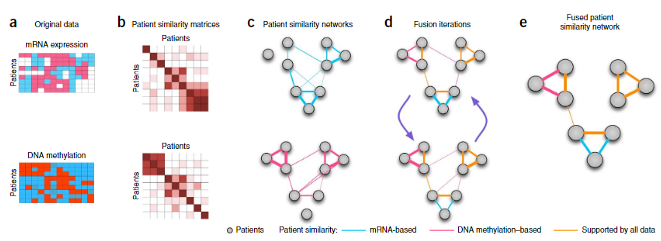
\includegraphics[scale=.53]{SNF.png}
	\caption{SNF processes \cite{wang2014similarity}:
	A detailed example of SNF steps. (a) An example representation of chemical structure feature and off-label side effect feature for the same set of drugs. (b) Drug-drug similarity matrices for each feature type. (c) Drug-drug similarity networks, equivalent to the drug-drug data. Nodes represent drugs, and edges represent drug pairwise similarities. (d) Network fusion by SNF iteratively updates each of the networks with information from the other networks, making them more similar with each step. (e) The iterative network fusion results in convergence to the final fused network. Edge color indicates which data type has contributed to the given similarity. }
	\label{SNF}
\end{figure}

In this section, using the similarity network fusion method that has described above, similarity matrices of the chemical structure and the off-label side effect of drugs were integrated. The output of this integration is a new similarity matrix of $S_{snf}$ with dimensions of $568 \times 568$, and elements of $S_{snf}$ have a value between zero and one.To integrate the network similarity, the package of SNFPy is used, which is implemented in Python and is available at \cite{SNFPy2020}.

\subsubsection*{Input matrix format}

At this stage, a matrix forms with 1139 columns and 322056 rows, which consists of the following columns:

1) Drug pairs: Name of the drug i-th and the name of the drug j-th.

2) Type of interaction: degressive (-1), enhancive (+1), and unknown (0).

3) The similarity vector of i-th drug from the $S_{snf}$ matrix with 568 elements.

4) The similarity vector of j-th drug from the $S_{snf}$ matrix with 568 elements.

Figure of \ref{BMatHeader} shows the header of matrix.

\begin{figure}[!h]
	\centering
	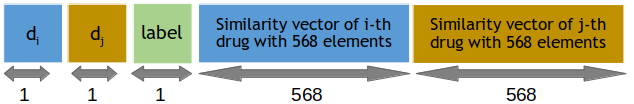
\includegraphics[scale=.53]{MatrixheaderB.png}
	\caption{Matrix header of B}
	\label{BMatHeader}
\end{figure}

We have 568 drugs, and the interaction of each drug with itself is meaningless. On the other hand, the drug pairs of $(d_i, d_j)$ and $(d_j, d_i)$ have the same label, while the corresponding similarity vectors of drugs in the drug pairs have been displaced. So, these drug pairs are dual. Both of them in the data augment the training data, which increases the model's ability to have a better prediction. As a result, the resulting matrix has 322056 data samples or rows ($(568 \times 568) - 568 = 322056$). According to the explanations provided, a matrix with dimensions of $322056 \times 1139$ is formed to input into our model, which is called $B$.


\subsection*{Devising of Recommender System}
In the previous steps, data was prepared to input any learning machine, including deep learning machines. But before presenting the model and inputting the data into the machine, one important point must be considered. As mentioned before, in this approach and other approaches, the positive and negative data have a specific label. While the zero label does not mean that there is no interaction between a pair of drugs, it does indicate that no interaction has yet been found for this pair of drugs. In the following, we present a method for detecting pairs of non-interacting drugs. Then we use these pairs of drugs as zero-labeled data in the next training.

\subsection*{Assessment}
K-Fold cross-validation (CV) is a well-proven approach to verify the algorithms' accuracy, model selection, and feature engineering in machine learning. To demonstrate that the feature set is informative enough, the selected model is robust and confident or the method has proper accuracy in comparison with other methods, the CV equation must be carefully designed. The production of test and experimental samples is as follows:

The whole data set has divided into K equal parts with consideration of dual pairs. Since biologically, the $(d_i, d_j)$ and $(d_j, d_i)$ drug pairs are the same we expect the model to predict their labels similarly.  in the separation of training and testing data, necessarily a drug pair and its dual are in the same group to prevent unfair results. The K-1 parts are used as a training data set, and the model has built based on them, and the test has performed with a remaining part. This procedure has repeated K times so that each of the K parts has used only once for testing, and each time accuracy has calculated for the constructed model. In this method, the average prediction accuracy in all K rounds is taken as the final accuracy for the classifier. The most common value for K in scientific literary is 5 or 10. Obviously, the more detailed validation in the K-fold CV the more reliable the classifier accuracy, the more comprehensive the obtained knowledge, and the more time-consuming the validation process.


\subsection*{Evaluation criteria}
In this study, we classify drug pairs into three classes, according to the type of interaction or non-interaction, so in order to compare the method performance with other existing methods, four measurement criteria, F- measure, accuracy, Area Under Roc Curve(AUC), and Area Under Precision-Recall Curve(AUPR) are Used. To define these criteria, at first, introduced four counting criteria in table
\ref{confusion_matrix_enh_deg}.

\begin{table}[h!]
	\centering
	\begin{tabular}{|c|c|c|c|}
		\cline{3-4}
		\multicolumn{2}{c}{}&\multicolumn{2}{|c|}{}\\
		\multicolumn{2}{c}{}&\multicolumn{2}{|c|}{Actual label}\\
		\multicolumn{2}{c}{}&\multicolumn{2}{|c|}{}\\
		\cline{3-4}
		\multicolumn{2}{c|}{}&&\\
		\multicolumn{2}{c|}{} & Actual Enhancive & Actual Degressive \\
		\multicolumn{2}{c|}{}&&\\
		\cline{1-4}
		&&&\\
		\multirow{5}{*}{Classifier Label} & Classified Enhancive & $T_{Enh}$ -- $cell_1$	 & $F_{Enh}$ -- $cell_2$\\
		&&&\\
		\cline{2-4}
		&&&\\
		&Classified Degressive & $F_{Deg}$ -- $cell_4$ & $T_{Deg}$ -- $cell_5$\\
		&&&\\
		\cline{1-4}
	\end{tabular}
	\newline
	\caption{The confusion matrix and relevant evaluation index.True Positive (TP): The number of residues classified as interacting correctly, False Positive (FP): The number of residues classified as interacting correctly incorrectly, False Negative (FN): The number of residues classified as non-interacting incorrectly, True Negative (TN): The number of residues classified as non-interacting correctly.}
	\label{confusion_matrix_enh_deg}
\end{table}

The table of shows confusion matrix of three classes. In this mode we have to modify the definitions of TP, TF, TN and TP versuse , as well as accuracy, precision, recall, \ref{confusion_matrix_temp}By using table \ref{confusion_matrix_temp}, four evaluation criteria are defined in the following order:

Accuracy: The fraction of all correct predictions (TP and TN) to all predictions.
$$ \mbox{Acurracy} =  \frac{ \mbox{TP} + \mbox{TN}}{\mbox{ all predicted interactions}} $$

Precision:The fraction of correct predicted interactions among all predicted interactions.
$$ \mbox{Precision} =  \frac{\mbox{TP}}{\mbox{TP} + \mbox{FP}} $$

Recall:The fraction of correct predicted interactions among all true interactions.
$$ \mbox{Recall} =  \frac{ \mbox{TP}}{\mbox{TP} + \mbox{FN}} $$
Precision and recall have a trade-off; thus, improving one of them may lead to a reduction in another.Therefore, utilizing F-measure, is more reasonable.

F-measure:the geometric mean of precision and recall.
$$ F-measure = \frac{ 2\times \mbox{Precision} \times \mbox{Recall}}{\mbox{Precision} + \mbox{Recall}} $$

It should be noted that if the interaction of two drugs is assigned to zero, it denotes that no evidence of their interaction has been found yet; thus, they may interact with each other. So we cannot identify TN and FP pairs correctly. The training process requires both interaction and non-interaction samples. Therefore, some of the zero assigned pairs are considered as non-interactive pairs in the training model. So every method may have some FP in its evaluations. This leads to a reduction in calculated precision and F-measure, while the real values of precision and F-measure may be higher.

Since the values of precision, recall, and F-measure is dependent on the value of the threshold, we also evaluate methods via AUC which is the area under the receiver operating characteristic (ROC) curve, and AUPR, that is the area under the precision-recall curve. These criteria indicate the efficiency of methods independent of the threshold value. In cases that the fraction of negative samples and positive samples are not equal, AUPR is the fairer criterion for evaluation.

\subsection*{Selecting and training model on known interactions}
To solve this problem, it is necessary to provide a model that detects non-interaction with high accuracy and confidence. Therefore, we design a model based on deep learning that predicts the possible non-interaction drug pairs and then use it to design a three-class model. Obviously, high accuracy in detecting these zeros can help provide a more accurate and confident three-class model.


\subsection*{Selecting model
\label{Selecting model}}
We separated rows of matrix B that contain positive and negative interactions. The new matrix contains 42,702 pairs of drugs with degressive and enhancive interactions. This data was used to train and find a more suitable model and found a stronger model among many models with different network structures. The final model was a deep neural network that used convolutional and fully connected layers. The features of all interactions (+1 and -1) contain 1136 features. We first divide these features into 10 equal parts. Then, in a 10-cycle for, each period we consider 1 part as testing data and the other 9 parts as a set of training data. We select different models and train the model in the 10-fold CV with 90  of the data. Then we test the model on the remaining 10 percent of the data. In the separating process, pairs of drugs dual are considered. Since the $ (d_i, d_j) $ and $ (d_j, d_i) $ pairs of drugs are not biologically different from each other, in the separation of training and testing data, necessarily a pair of drugs and their dual are in the same group. This prevents unfair results.

After testing the different structures, we have modeled the final deep neural network shown in Figure
\ref{CNNModel}.
\begin{figure}[!h]
	\centering
	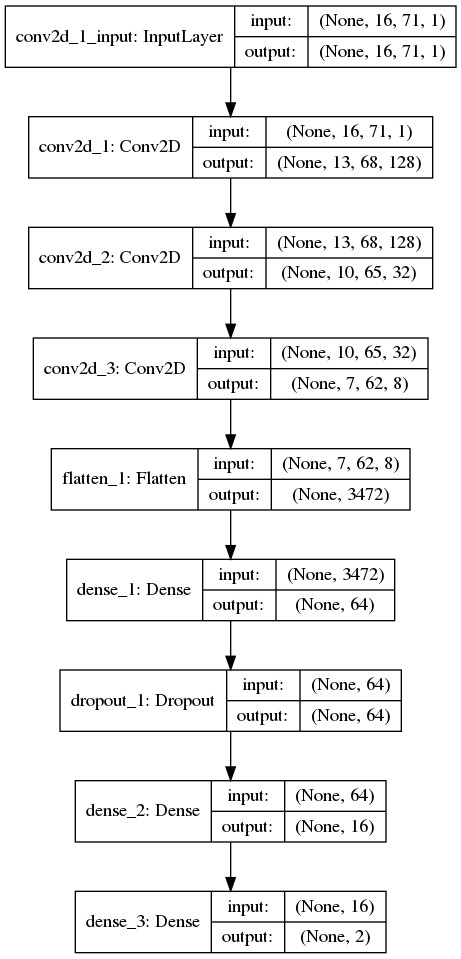
\includegraphics[scale=0.4]{ModelSelection/model.jpg}
	\caption{The arrangement of the neural network layers for detecting possible zeros}
	\label{CNNModel}
\end{figure}

This network has three layers of two-dimensional convolution. In the following, there are three fully connected convolution layers. The last layer has two outputs for predicting degressive or enhancive interaction. Convolution layers have 4-dimensions square filters with a Stride of 1. Each convolution layer also has a Rectified Linear Units (ReLU) activation function \cite{nair2010rectified}, which is defined as the positive part of its argument:

\begin{equation}
	\begin{aligned}
		ReLU(x) = max \{x, 0\}
	\end{aligned}
\end{equation}

The number of convolution filters is 128, 32, and 8, respectively. All connected layers have 64, 16, and 2 nodes, respectively. The first two layers have the activation function of ReLU, and the last layer with 2 nodes has a Sigmoid activation function \cite{hinton2012deep}, which is calculated as follows:

\begin{equation}
	\begin{aligned}
		Sigmoid(x) = \dfrac{1}{1 + e^{-x}}
	\end{aligned}
\end{equation}

Convolution layers using a Flatten layer Connects to fully connected layers. The function of this layer is to transform a two-dimensional matrix into a one-dimensional vector. The output of this input layer of the first layer is fully connected. Also, between fully connected 64 and 16 nodes, we used one Dropout layer \cite{srivastava2014dropout} with a wast value of 0.2. This value indicates that the network in this layer does not randomly consider 20 percent of the features. This layer is used to prevent over-fitting of the model and forces the model to extract and use more features with more confidence for prediction. If some of them are removed, the algorithm's prediction power either doesn't decrease or doesn't rely on a few specific features.

Our studies and trials have shown that two-dimensional convolution layers work better than their one-dimensional counterparts because in this case, the filters can detect more drug similarities, and it is possible to extract more powerful Features. Therefore, the 1136-dimension  feature vectors are transformed into matrices with dimensions of $ 71 \ $ 16 times. Figure
\ref{paramNumber1} 
shows the number of learnable weights for each layer. Also, the total number of weights is calculated, which indicates the general complexity of the model.

\begin{figure}[!h]
	\centering
	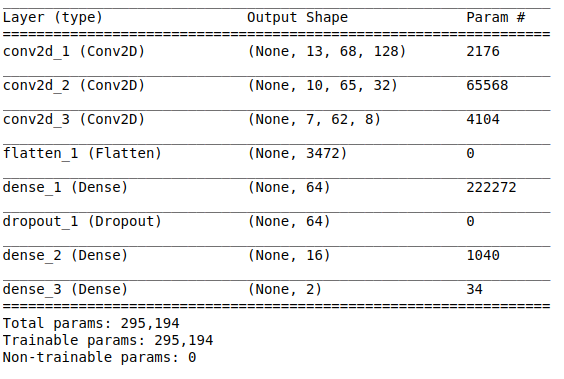
\includegraphics[scale=0.65]{ModelSelection/modelparameters.png}
	\caption{Learnable parameters of two-class Neural Networks}
	\label{paramNumber1}
\end{figure}

The following settings are used in the construction of the convolution neural network:

1) We used Tensorflow \cite{abadi2016tensorflow} (version 1.14.0) and KERAS \cite{chollet2015keras} (version 2.2.5) packages to implement the neural network.

2) The categorical-cross entropy loss function was considered an objective function for the neural network, which is generally used to train a classification network \cite{ghosal1997your, toda2012research, seen20121}.

3) ADAM optimization \cite{kingma2014adam} was used to manipulate the neural network weights to find a promising optimal (minimum) state of the loss function.

4) The number of epochs was considered 5.

5) Learning rate of $1.0 \times 10^{-5}$ was used.

Keep in mind that this network's hyperparameters are not optimized, and the specified parameters are not necessarily at their best. There are two reasons for not optimizing hyperparameters:

1) Model overfitting: If hyperparameters changed to the best values, it is expected that the model will get better results on the present data, but there is no guarantee that the extracted features by the model are significant and works well when used in new cases. In this case, the so-called model is over-fitted and will be a negative point for the model.

2) Robustness: Optimal hyperparameters give better results for the present data, but different drug similarities may be used in the future, or new data may be collected, and the present results may not be repeated. In this case, the model loses its robustness and will not be accepted in the pharmaceutical and pharmacological community.

Finally, we examine the results of the proposed model in the 10-fold CV from three views:

1)Accuracy: In a 10-fold CV,the model obtained $AUC=0.97 , AUPR=0.93$ for degressive interactions , and $AUC=0.97,AUPR=0.99 $ for enhansive interactions. These results indicate the high accuracy and detection power of the model.

2) Variance: The confidence interval for the reported values with a reliability coefficient above 95 percent was narrow and close to each other. Out of four reported confidence interval values, three values were less than $\pm 0.002$, and only for the degressive interaction, the AUPR was in the range of $\pm 0.005$. The low amount of variance obtained from the model shows that the proposed model is robust.

3) Resolution capability: By plotting the output probability distribution diagram, as shown in Figure \ref{DDIProbHist}, it is clear that values +1 and -1 are well separated, and probability distribution degressive and enhancive have slightly Subscriptions.

\begin{figure}[!h]
	\centering
	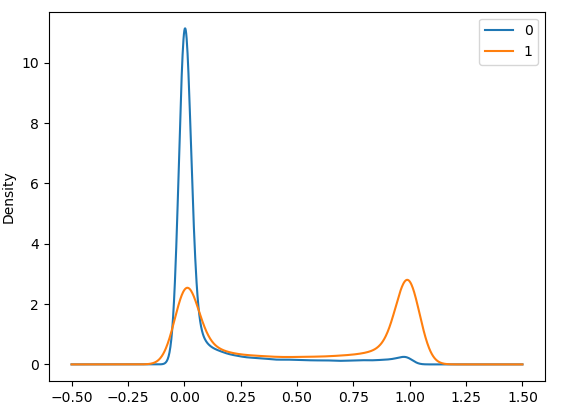
\includegraphics[scale=0.5]{ModelSelection/densityDegEnh.png}
	\caption{probability density distribution diagram of Degressive and enhancive. In this figure, 0 is the same as the $-1$label, and 1 is the same as $+1$.}
	\label{DDIProbHist}
\end{figure}

The Suducode \ref{modelSelectionSuducode} shows the step-by-step model selection process.

\renewcommand{\algorithmicrequire}{\textbf{Input:}}
\renewcommand{\algorithmicensure}{\textbf{Output:}}
\begin{algorithm}[!h]
\caption{Model selection suducode}
\label{modelSelectionSuducode}
\begin{algorithmic}[1]
\REQUIRE
+1 and -1 drug pairs features  
\ENSURE 
+1 and -1 diagnostic model
\vskip.5\baselineskip\hrule height 0.4pt\vskip.5\baselineskip

\STATE
Apply 10-fold CV to the features of +1 and -1 drug pairs.

\STATE
Select the right model. 

\STATE
Test the model results in 10-fold CV.
 
\STATE
If 3 is correct then select the model, else go to 2. 

\end{algorithmic}
\end{algorithm}


\subsection*{Detecting of non-interaction drug pairs}
In the previous step, a high-precision, robust, and accurate model has been presented to detect drug pairs' potential interactions for both degressive and enhancive. Therefore, this model has the ability to detect non-interactions (real zeros) as follows. If drug pairs are unlikely to interact, then those drug pairs are likely to be real zeros.

According to this hypothesis, the model was used to predict all unknown drug pairs (zeros). Unknown drug pairs include 270,000 drug pairs. We consider drug pairs as non-interacting drug pairs in the model's output if the enhancive and degressive probability are less than 0.4 and 0.4. Among the unlabeled data, about 65,000 drug pairs had these conditions. These drug pairs are candidates for non-interaction. Due to the model's high accuracy, the low variance of results, and the model's high resolution, we consider these pairs non-interaction drug pairs.

\subsection*{Selecting and training model on known and unknown interactions}
This section uses known data and potential non-interaction candidates to form a data set. Here, we use the non-interaction candidate drug pairs as real zeros. The recommender system presented in Section \ref{Selecting model} is also used for the final model.

First, the B matrix rows, which contain the +1 and -1 interactions, are separated according to the previously detailed procedure and placed in 10 parts. Then, 30,000 non-interacting candidate drug pairs were randomly selected from 65,000 drug pairs. In the chosen drug pairs, the drug pairs and the dual of them must be non-interaction candidates. The zeros group is randomly divided into 10 parts, so each drug pairs and the dual are in the same batch. Then 10 parts of zeros are merged with 10 parts of pre-prepared +1s and -1s. 

The data set contains approximately 72,702 drug pairs, divided into relatively equal parts, is ready to use in the training and testing of the final recommender system.

\subsection*{Selecting final model}
The final model is almost the same as that described in Section
\ref{Selecting model}. That means it has three Conv-layer with 128, 32, and 8 filters. Then, as before, three fully connected Conv layers were used. The difference was that the number of nodes changed from 64, 16 and 2 to 64, 16, and 3 in each layer, respectively. Specifically, this model gives three possible outputs for the three modes of enhancive interaction, non-interaction, and depressive interaction. Also, the number of epochs was considered 9. The deep neural network model for predicting interaction is shown in Figure
\ref{Triple_model}. At this stage, the new model was not chosen because:

1) The power of this model for relatively accurate detection of enhancive and degressive interactions has been proven.

2) The zeros used in this section are just suggested and have not been approved by the Pharmacology Laboratory. Until the writing of this article, a comprehensive database for non-interaction cases has not been made public. If the model selection is made again, a model may be selected that is not necessarily valid in real-world application and hard to accept.

Due to the above reasons, the zeros recommender system is used to comprehensive drug-drug interactions prediction by changing the number of outputs from 2 to 3 as the input data. The proposed SNF-CNN method's general process is presented in the form of pseudocode \ref{SNFCNNSuducode}, which includes the steps of preparation, model selection, real zero detection, and the presentation of a comprehensive recommender system.

\begin{figure}[!h]
	\centering
	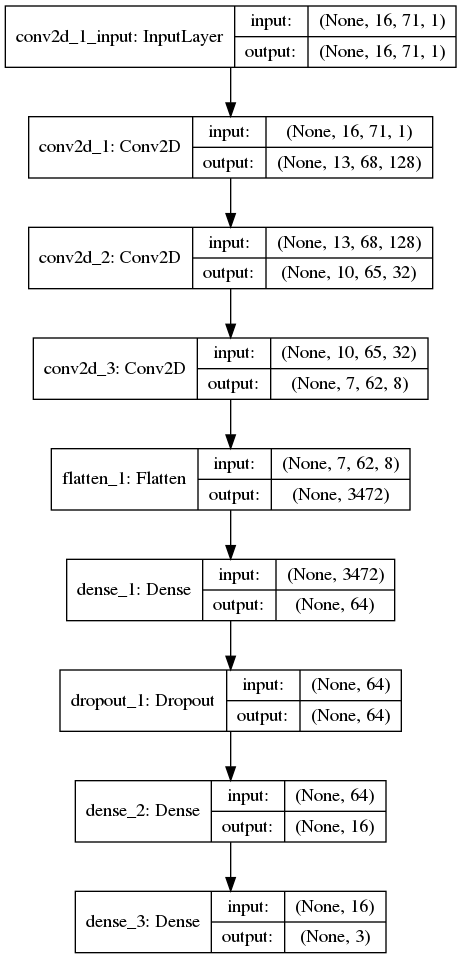
\includegraphics[scale=0.43]{lastTripleModel/modelTripleLayers.png}
	\caption{Arrangement of neural network layers SNF-CNN Predict triple-class interaction. Non-interaction (0), degressive interaction (-1) and enhancive interaction (+1)}
	\label{Triple_model}
\end{figure}

\renewcommand{\algorithmicrequire}{\textbf{Input:}}
\renewcommand{\algorithmicensure}{\textbf{Output:}}
\begin{algorithm}[!h]
\caption{Final model selection(SNF-CNN) suducode}
\label{SNFCNNSuducode}
\begin{algorithmic}[1]
\REQUIRE
Drug pairs features(+1,-1,real 0)  
\ENSURE
Diagnostic model for interaction and non-interaction
\vskip.5\baselineskip\hrule height 0.4pt\vskip.5\baselineskip

\STATE
Calculate drug similarity matrices with the cosine method. 

\STATE 
Integrate drug similarity matrices with the similarity network fusion(SNF) method.

\STATE
Built the input matrix of the model. 

\STATE
Select the fit known interactions model and train it.

\STATE
Predict probable zeros by using step 4.

\STATE
Select the fit known interactions and zeros of step 5 model , and train it.

\STATE
Predict on unknown drug pairs.

\end{algorithmic}
\end{algorithm}


\section*{Result and discussion}

Each setting of model and features and each data set needs its own validation process. According to the type of problem and the methods, we use two types of 10-fold CV to select the most proper model also to validate the results of the chosen model. The metrics which are used in validation are described in following.

\subsection*{Evaluation criteria}
In this study, we classify drug pairs into three classes, according to the type of interaction or non-interaction, so in order to compare the method performance with other existing methods, four measurement criteria, F- measure, accuracy, Area Under Roc Curve(AUC), and Area Under Precision-Recall Curve(AUPR) are Used. To define these criteria, at first, introduced four counting criteria in table
\ref{confusion_matrix_temp}.

\begin{table}[h!]
	\centering
	\begin{tabular}{|c|c|c|c|c|}
		\cline{3-5}
		\multicolumn{2}{c}{}&\multicolumn{3}{|c|}{}\\
		\multicolumn{2}{c}{}&\multicolumn{3}{|c|}{Actual label}\\
		\multicolumn{2}{c}{}&\multicolumn{3}{|c|}{}\\
		\cline{3-5}
		\multicolumn{2}{c|}{}&&&\\
		\multicolumn{2}{c|}{} & Actual Enhancive & Actual Degressive & Actual Non-interaction\\
		\multicolumn{2}{c|}{}&&&\\
		\cline{1-5}
		&&&&\\
		\multirow{7}{*}{Classifier Label} & Classified Enhancive & $T_{Enh}$ -- $cell_1$	 & $F_{Enh}$ -- $cell_2$&$F_{Enh}$ -- $cell_3$\\
		&&&&\\
		\cline{2-5}
		&&&&\\
		&Classified Degressive & $F_{Deg}$ -- $cell_4$ & $T_{Deg}$ -- $cell_5$&$F_{Deg}$ -- $cell_6$\\
		&&&&\\
		\cline{2-5}
		&&&&\\
		&Classified Non-interaction &$F_{N-Int}$ -- $cell_7$&$F_{N-Int}$ -- $cell_8$&$T_{N-Int}$ -- $cell_9$\\
		&&&&\\
		\cline{1-5}
	\end{tabular}
	\newline
	\caption{The confusion matrix and relevant evaluation index.True Positive (TP): The number of residues classified as interacting correctly, False Positive (FP): The number of residues classified as interacting correctly incorrectly, False Negative (FN): The number of residues classified as non-interacting incorrectly, True Negative (TN): The number of residues classified as non-interacting correctly.}
	\label{confusion_matrix_temp}
\end{table}

The table of shows confusion matrix of three classes. In this mode we have to modify the definitions of TP, TF, TN and TP versuse , as well as accuracy, precision, recall, \ref{confusion_matrix_temp}By using table \ref{confusion_matrix_temp}, four evaluation criteria are defined in the following order:

Accuracy: The fraction of all correct predictions (TP and TN) to all predictions.
$$ \mbox{Acurracy} =  \frac{ \mbox{TP} + \mbox{TN}}{\mbox{ all predicted interactions}} $$

Precision:The fraction of correct predicted interactions among all predicted interactions.
$$ \mbox{Precision} =  \frac{\mbox{TP}}{\mbox{TP} + \mbox{FP}} $$

Recall:The fraction of correct predicted interactions among all true interactions.
$$ \mbox{Recall} =  \frac{ \mbox{TP}}{\mbox{TP} + \mbox{FN}} $$
Precision and recall have a trade-off; thus, improving one of them may lead to a reduction in another.Therefore, utilizing F-measure, is more reasonable.

F-measure:the geometric mean of precision and recall.
$$ F-measure = \frac{ 2\times \mbox{Precision} \times \mbox{Recall}}{\mbox{Precision} + \mbox{Recall}} $$

It should be noted that if the interaction of two drugs is assigned to zero, it denotes that no evidence of their interaction has been found yet; thus, they may interact with each other. So we cannot identify TN and FP pairs correctly. The training process requires both interaction and non-interaction samples. Therefore, some of the zero assigned pairs are considered as non-interactive pairs in the training model. So every method may have some FP in its evaluations. This leads to a reduction in calculated precision and F-measure, while the real values of precision and F-measure may be higher.

Since the values of precision, recall, and F-measure is dependent on the value of the threshold, we also evaluate methods via AUC which is the area under the receiver operating characteristic (ROC) curve, and AUPR, that is the area under the precision-recall curve. These criteria indicate the efficiency of methods independent of the threshold value. In cases that the fraction of negative samples and positive samples are not equal, AUPR is the fairer criterion for evaluation.

%$$ \mbox{TPR} = \frac{ \mbox{TP}}{\mbox{TP} + \mbox{FN}} $$ 


%$$ \mbox{FPR} =  \frac{ \mbox{FP}}{\mbox{FP} + \mbox{TN}} $$



\subsection*{First case: 10-fold CV without unknown interactions}
In this case, we randomly select 90 percent of the enhancive and degressive interactions. For the testing set, we consider the remaining 10 percent of the enhancive and degressive interactions. In the first case of the testing procedure,  the model was selected, and some hyper-parameters, such as the number of epochs, were determined.Figure \ref{ModelSelection}, shows the training process for the selected model. As expected, the model's accuracy is strict on ascending training data, but there are ups and downs for testing data after Epoch 5. In the loss function graph, by the end of epoch 5, as the epochs increase, the loss function's value on training and testing procedure decreases. After epoch 5, the trend of training data continues, but the testing trend is reversed. In other words, over feet occurs. Therefore, based on the graphs, the appropriate number of epochs in this step was considered 5.
\begin{figure}[!h]
	%\centering
	\begin{minipage}{1\linewidth} 
		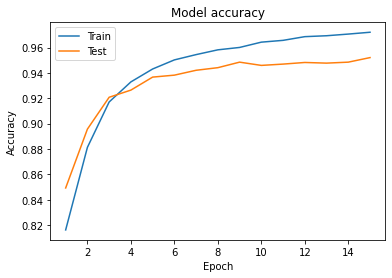
\includegraphics[width=.48\textwidth]{ModelSelection/selectedModelAcc.png} 
		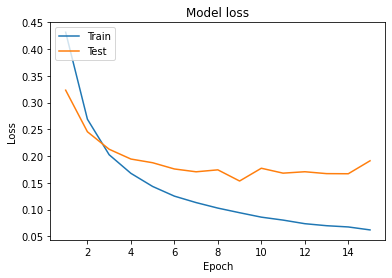
\includegraphics[width=.48\textwidth]{ModelSelection/selectedModelLoss.png} 
	\end{minipage}
	\caption{\textbf{Accuracy and loss function for the binary model:} The right figure shows the model's accuracy on training and validation data during 15 epochs, and the left figure shows the loss function values at different epochs.}
	\label{ModelSelection}
\end{figure}
\subsubsection*{Second case: 10-fold CV with unknown interactions}
In this case, we divide the set of all interactions (enhancive, degressive, and zeros of the first step) into 10 equal parts. We consider one part of the testing set and the other 9 parts as the training data set. Divide all the zeros in the previous step into 10 parts and add a 1 to 9 ratio to both testing and training sets. In the second case, the previous model's 10-fold CV procedure was trained with the least changes to predict the three classes. Besides, hyper-parameter, the number of epochs was determined. Figure
\ref{lastTripleModel} 

It shows the training process. The process of the accuracy of the model on training data increases steadily with the increase of epochs. Still, the model after epoch 9 reduces a constant and decreases the accuracy a little for testing data.

\begin{figure}[!h]
	%\centering
	\begin{minipage}{1\linewidth}
		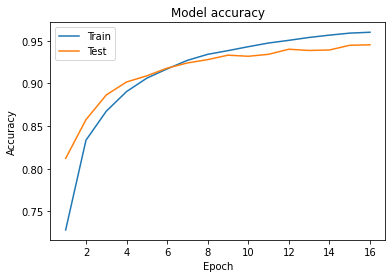
\includegraphics[width=.48\textwidth]{lastTripleModel/modelTripleACC.png}
		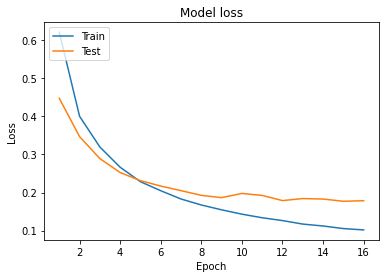
\includegraphics[width=.48\textwidth]{lastTripleModel/modelTripleLoss.png}
	\end{minipage}
	\caption{\textbf{Accuracy and loss function diagrams for the triple model:} The right figure shows the accuracy of the model on training and validation data during 16 epochs, and the left figure shows the loss function values at different epochs.}
	\label{lastTripleModel}
\end{figure}


\section*{Comparison of results}
Based on the validation procedure described in Section
\ref{K-fold CV}
, the interaction type detection model was selected and trained. Then, the final three-class model was presented by recognizing the most probable non-interactions. So we tested the SNF-CNN model on data to check the evaluation, robustness, and efficiency of the CV. Results SNF-CNN and other methods for comparison are presented and discussed in this section. Before comparing the different methods, an example of the results of neural network implementation is presented to identify the type of degressive and enhancive interactions.

\begin{table}[h!]
\centering
\begin{tabular}{|c|c|c|c|c|}
\hline
& Precision & Recall & F-measure & Support \\
\hline
Degressive & 0.94 & 0.83 & 0.88 & 850 \\
\hline
Enhancive & 0.95 & 0.99 & 0.97 & 3052 \\
\hline
Accuracy &  & & 0.95 &3902\\
\hline
Macro Avg & 0.95 & 0.91 & 0.93 & 3902\\
\hline
Weighted Avg & 0.95 & 0.95 &0.95 & 3902\\
\hline
\end{tabular}
\newline
	\caption{Interaction type classification report}
	\label{classificatonReport}
\end{table}

Table
\ref{classificatonReport}
an example of a model implementation result is the ability of the model in terms of precision, recall and F-measure Indicates the type of interactions. According to table
\ref{classificatonReport}
the precision of the model in detecting enhancive and degressive interactions is 95 percent and 94 percent, while recall is 99 percent and 83 percent, respectively. the F-measure is also 97  percent and 88 percent that the higher ability of the model to detect degressive interactions comes from a higher number of these types of interactions. The ratio of degressive interaction to enhancive interaction is approximately 4 to 1.

\begin{table}[h!]
\centering
\begin{tabular}{|c|c|c|c|c|}
\hline
& Precision & Recall & F-measure & Support  \\
\hline
Enhancive & 0.88 & 0.84 & 0.86 & 850\\
\hline
Non-intraction & 0.96 & 0.95 & 0.96 & 3000\\
\hline
Degressive & 0.95 & 0.97 & 0.96 & 3052\\
\hline
Accuracy &  & & 0.95 &6902\\
\hline
Macro Avg & 0.93 & 0.92 & 0.93 & 6902 \\
\hline
Weighted Avg & 0.95 & 0.95 &0.95 & 6902\\
\hline
\end{tabular}
\newline
	\caption{Three-Classes interaction classification report}
	\label{TripleclassificatonReport}
\end{table}

Also in the table
\ref{TripleclassificatonReport}
three-Classes interaction classification is displayed. In this implementation, the accuracy of the model for detecting degressive interaction, non-interaction, and enhancive interaction is 95 percent, 96 percent, and 88 percent, respectively. The recall is 97 percent, 95 percent, and 84 percent, respectively, and finally F-measure It is 96, 96, and 86 percent. In comparison, the model power in the three-classes decreases slightly to the two-classes, which can be due to two reasons.

1) The problem of three-classes is more difficult than two-classes.

2) Zeros or non-interaction are not necessarily real and are not pharmacologically proven, so there is a possibility of some disturbance.

For the above reasons, some reduction in the power of the three-classes model in detection was not unexpected.

\begin{table}[h!]
\centering 
\begin{tabular}{|c|c|c|c|}
\hline
& AUC & AUPR\\
\hline
degressive	& $0.9747 \pm 0.0033$ & $0.9666 \pm 0.0045$\\
\hline
enhancive  & $0.9686 \pm 0.0028$ & $0.8221 \pm 0.0184$\\
\hline
non-interaction & $0.9714 \pm 0.0040$ & $0.9480 \pm 0.0083$\\
\hline
\end{tabular}
\newline
	\caption{Results of SNF-CNN algorithm in predicting three-classes based on AUC and AUPR criteria and their confidence interval}
	\label{SNF-CNNresult}
\end{table}

Since the previous algorithms in the three-classes prediction of DDI used AUC and AUPR therefore, the results of the proposed algorithm are based on these two criteria according to table
\ref{SNF-CNNresult}.Also in table
\ref{SNF-CNNresult}
for the algorithm presented in this research, high and low intervals are reported with 95 percent confidence, which shows that the results of the algorithm have slightly changed in the 10- fold CV and the proposed algorithm is robust and reliable.

\begin{table}[h!]
\centering 
\begin{tabular}{|c|c|c|c|}
\hline
& AUC	& AUPR \\
\hline
SNF-CNN	& 0.971 & 0.912\\
\hline
BRSNMF\cite{shi2019detecting}  & 0.805 & 0.644\\
\hline
Semi-NMF \cite{yu2018predicting} & 0.796 & 0.579\\
\hline
TMFUF\cite{shi2018tmfuf}   & 0.842  & 0.526\\
\hline
\end{tabular}
\newline 
	\caption{Comparison of the results of three-classes prediction algorithms based on criteria AUC and AUPR}
	\label{AUCAUPR}
\end{table}

In the table
\ref{AUCAUPR}
results of SNF-CNN averaged for the three classes and compared with other existing three-classes algorithms. According to the table
\ref{AUCAUPR} the proposed algorithm has a high difference compared to other superior algorithms with the problem of ternary and has been able to challenge other algorithms.


\section*{Conclusions}
Existing computational approaches are able to present potential large-scale interactions before using drugs on the market. However, they cannot predict comprehensive interactions, including degressive and enhancive interactions. It is more useful to know whether or not a drug pair is enhancive DDI or a degressive DDI  than to know whether or not a drug pair is DDI. Without considering the pharmacological changes caused by DDIs, most existing approaches only report two-classes prediction.  In addition, the occurrence of degressive and enhancive DDIs is not random, but none of the existing approaches investigates and leverages this intrinsic important property of interactions when treating complex diseases (including treatment with three or more drugs).

In this work, after representing a comprehensive DDI network, we used the structure of recommender systems to design a novel algorithm. Although the prediction obtained by the new algorithm is inspiring, overall performance can still be improved. For this reason, we investigate those incorrectly predicted DDIs. After checking them case-by-case, and in order to prove the algorithm in practice, check the prediction performance of the algorithm in the latest version of the DrugBank database. Observations and investigations led to the discovery of three reasons for wrong predictions:

The first is named as false-positive drug pairs, which are precisely labeled as DDIs in DrugBank version 4, but in the current version, they are correctly labeled as non-DDIs. For example, the old version of DrugBank records that Apraclonidine ( a Sympathomimetic drug used in glaucoma therapy) increases the atrioventricular blocking activities of Alprenolol and Bevantolol, while the newer version removes it.

The second one is false-negative drug Pairs, which are wrongly labeled as non-DDIs in DrugBank version 4  but in the current version, they are reported as DDIs.For example, the pair of Valrubicin and Cyclosporine as well as the pair of Ergocalciferol and  Calcitriol in the newer version of DrugBank reports, Valrubicin (bladder cancer treatment drug) Increases the activity of the nephrotoxic drug Cyclosporine(A drug that suppresses the immune system with a special action on T-lymphocytes), while the combined therapy of Calcitriol and Ergocalciferol increases the risk or severity of adverse effects in the multiple-drug therapy.

The last one refers to change Pair DDIs, which are labeled as enhancive DDIs in DrugBank version 4, but in the current version, are labeled as degressive DDIs, and vice versa.

It is anticipated that the SNF-CNN approach, will be able to achieve better DDI prediction by the better datasets with fewer of both false-positive and false-negative drug pairs. For future work, it is recommended that the dataset always be collected from the latest version of DrugBank.

Three-classes data is an attempt to improve expression and problem solving over two-classes data. However, three-classes data does not have sufficient biological significance and provides limited biological information. This means that predicting the type of DDI can be useful, but it is not clear at what stage of the pharmacokinetic or pharmacodynamic stages this DDI occurred. Therefore, it is suggested to collect datasets with degressive and enhancive labels from each of the pharmacokinetic and pharmacodynamic steps. In this case, more meaningful models in terms of pharmacology and machine learning are taught. The resulting models are more important to pharmacists and pharmacists and will be more useful.

\section*{Appendix}
Text for this section\ldots

%%%%%%%%%%%%%%%%%%%%%%%%%%%%%%%%%%%%%%%%%%%%%%
%%                                          %%
%% Backmatter begins here                   %%
%%                                          %%
%%%%%%%%%%%%%%%%%%%%%%%%%%%%%%%%%%%%%%%%%%%%%%

\begin{backmatter}

\section*{Acknowledgements}%% if any
The author would like to thank the reviewers for their constructive comments that help make the paper much clearer.

\section*{Funding}%% if any
Text for this section\ldots

\section*{Abbreviations}%% if any
DDI:Drug-drug interactions; CV:cross-validation; SNF:Similarity Network Fusion; 

\section*{Availability of data and materials}%% if any
the code and data is available at GitHub page of \href{https://github.com/aminkhod/DDI-Project/tree/master/CNN\%20model\%20to\%20Recommend\%20Comperhancive\%20DDIs}{SNF-CNN code and data}


\section*{Ethics approval and consent to participate}%% if any
The authors declare that they have consenting to participate.

\section*{Competing interests}
The authors declare that they have no competing interests.

\section*{Consent for publication}%% if any
The authors declare that they have consenting to publication.

\section*{Authors' contributions}
Bl conceived and designed the experiments, draft the manuscript, and analyzed the results. MAK contributed materials/analysis tools and developed the codes used in the analysis. CE is the corresponding author. All authors read and approved the final manuscript.

%\section*{Authors' information}%% if any
%Text for this section\ldots
%%%%%%%%%%%%%%%%%%%%%%%%%%%%%%%%%%%%%%%%%%%%%%%%%%%%%%%%%%%%%
%%                  The Bibliography                       %%
%%                                                         %%
%%  Bmc_mathpys.bst  will be used to                       %%
%%  create a .BBL file for submission.                     %%
%%  After submission of the .TEX file,                     %%
%%  you will be prompted to submit your .BBL file.         %%
%%                                                         %%
%%                                                         %%
%%  Note that the displayed Bibliography will not          %%
%%  necessarily be rendered by Latex exactly as specified  %%
%%  in the online Instructions for Authors.                %%
%%                                                         %%
%%%%%%%%%%%%%%%%%%%%%%%%%%%%%%%%%%%%%%%%%%%%%%%%%%%%%%%%%%%%%

% if your bibliography is in bibtex format, use those commands:
\bibliography{bmc_article.bib}      % Bibliography file (usually '*.bib' )
\bibliographystyle{bmc-mathphys} % Style BST file (bmc-mathphys, vancouver, spbasic).

% for author-year bibliography (bmc-mathphys or spbasic)
% a) write to bib file (bmc-mathphys only)
% @settings{label, options="nameyear"}
% b) uncomment next line
%\nocite{label}

% or include bibliography directly:
% \begin{thebibliography}
% \bibitem{b1}
% \end{thebibliography}

%%%%%%%%%%%%%%%%%%%%%%%%%%%%%%%%%%%
%%                               %%
%% Figures                       %%
%%                               %%
%% NB: this is for captions and  %%
%% Titles. All graphics must be  %%
%% submitted separately and NOT  %%
%% included in the Tex document  %%
%%                               %%
%%%%%%%%%%%%%%%%%%%%%%%%%%%%%%%%%%%

%%
%% Do not use \listoffigures as most will included as separate files



\section*{Figures}
%\begin{figure}[h!]
%  \caption{Sample figure title}
%\end{figure}
%
%\begin{figure}[h!]
%  \caption{Sample figure title}
%\end{figure}

%%%%%%%%%%%%%%%%%%%%%%%%%%%%%%%%%%%
%%                               %%
%% Tables                        %%
%%                               %%
%%%%%%%%%%%%%%%%%%%%%%%%%%%%%%%%%%%

%% Use of \listoftables is discouraged.
%%
\section*{Tables}
%\begin{table}[h!]
%\caption{Sample table title. This is where the description of the table should go}
%  \begin{tabular}{cccc}
%    \hline
%    & B1  &B2   & B3\\ \hline
%    A1 & 0.1 & 0.2 & 0.3\\
%    A2 & ... & ..  & .\\
%    A3 & ..  & .   & .\\ \hline
%  \end{tabular}
%\end{table}


%%%%%%%%%%%%%%%%%%%%%%%%%%%%%%%%%%%
%%                               %%
%% Additional Files              %%
%%                               %%
%%%%%%%%%%%%%%%%%%%%%%%%%%%%%%%%%%%

\section*{Additional Files}
  \subsection*{Additional file 1 --- Sample additional file title}
    Additional file descriptions text (including details of how to
    view the file, if it is in a non-standard format or the file extension).  This might
    refer to a multi-page table or a figure.

  \subsection*{Additional file 2 --- Sample additional file title}
    Additional file descriptions text.

\end{backmatter}
\end{document}
